
% VLDB template version of 2020-08-03 enhances the ACM template, version 1.7.0:
% https://www.acm.org/publications/proceedings-template
% The ACM Latex guide provides further information about the ACM template

\documentclass[sigconf, nonacm]{acmart}

\begin{document}
\title{A Quick Analysis of a FOREX Trading System and its tendencies}

%%
%% The "author" command and its associated commands are used to define the authors and their affiliations.
\author{Ignacio Rus Prados}
\affiliation{%
  \institution{Ironhack Data Analytics Bootcamp}
  \city{Full time}
  \state{March 2021}
}
\email{enekorus@gmail.com}

\maketitle

\section{Introduction}

The foreign exchange market (FOREX, FX, or currency market) is a global decentralized market for the trading of currencies. This market determines foreign exchange rates for every currency. It includes all aspects of buying, selling and exchanging currencies at current or determined prices. In terms of trading volume, it is by far the largest market in the world, followed by the credit market. \\

The main participants in this market are the larger international banks. However, individual traders can also access the market and profit from smaller operations so long as their assessment of the risk for each of their predictions rightly compensates the amount they decide to invest in each operation. In order to success, they design trading systems that analyze different currency exchanges and estimate the risk and expected profit. These systems can be operated manually or automatically, providing the trader with instructions on whether they should start a new operation or not. \\

In our case, we'll be analyzing a trading system developed by Ramón Rosa Augusto, an independent trader that has been studying the currency market for several years.

\section{Data}

Once a trading system has been designed, we can start storing data of each operation the system has deemed as profitable. We have been assigned the task of analyzing a database that contains two measures for each operation that has been performed.\\

\begin{table}[hb]% h asks to places the floating element [h]ere.
  \caption{A quick look at our database structure}
  \label{tab:freq}
  \begin{tabular}{ccl}
    \toprule
    Date & Profit\\
    \midrule
    4/2/2018 & 0.76\\
    11/2/2018 & 0.50\\
    \cdot & \cdot\\
    \cdot & \cdot\\
    \cdot & \cdot\\
    20/4/2021 & -1\\
  \bottomrule
\end{tabular}
\end{table}

The first measure is the 'profit' or 'profit per unit invested', which represents how much profit we have made in each operation for each unit of currency invested.\\

The second measure is the date in which the operation was performed. Dates range from February 2018 to April 2021, although the amount of data is not evenly distributed throughout that time so a few comments should be made: this trading system is designed to work during what we could define as an academic year/period, i.e. from October to June. Therefore we won't find any operations during the summer period (July to September). Secondly, some periods of the year will be more active than others, specially when globally disruptive events such as an economic crisis or a global pandemic drastically raise the estimated risk for every operation, so gaps of data should be expected.\\


\section{Goals}

There are two main goals in this project: firstly, we want to study an observed change in tendency happening during the last part of what we have called Period 4. The goal is to determine whether this change is significant or if it is an expected deviation given the statistical nature of the system. Then we will examine the evolution of our system over time, concentrating on its performance during different months and periods, in order to find patterns that can help us optimize the system's performance.

\section{Analysis}
\subsection{First look}

Before we start a deeper analysis we should understand how our data looks like. A good way to start analyzing any trading system is by evaluating its cumulative profit sum for each new operation. This indicates how much profit per unit invested we have accumulated at a given point since we started investing. Therefore, this allows us to see if the system has a positive growth over time, which is what we expect from any system that works.\\

\begin{figure}
  \centering
  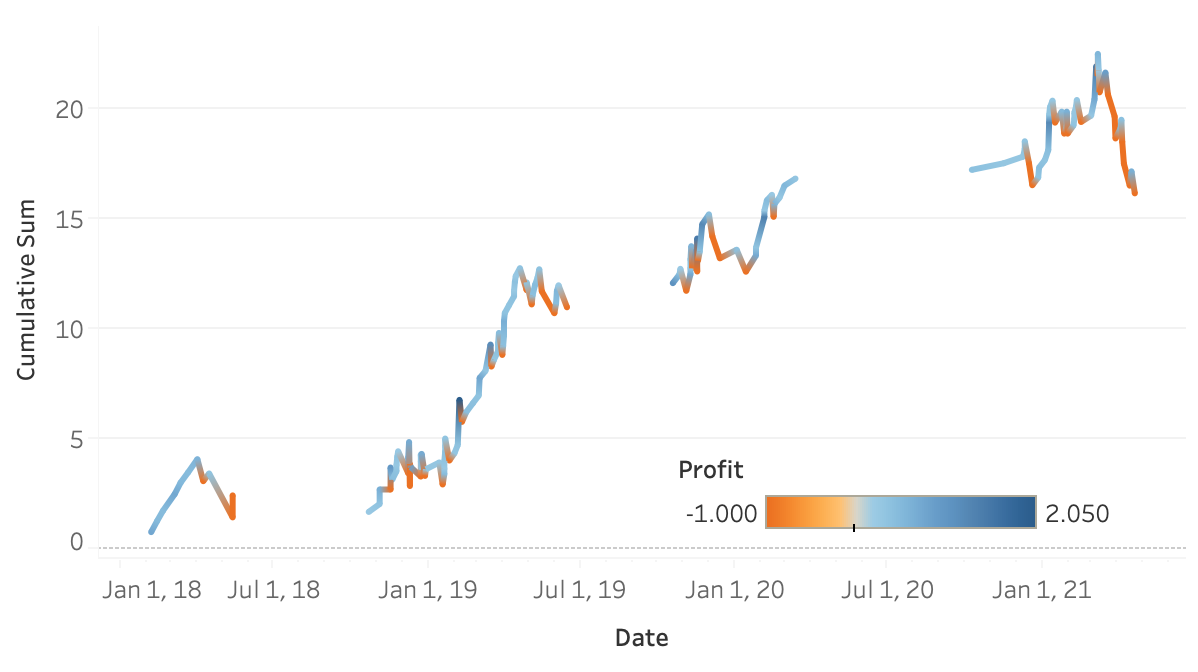
\includegraphics[width=\linewidth]{figures/pic1}
  \caption{The cumulative profit sum over time. Four separate periods can be observed with an overall positive growth}
  \label{fig:duck}
\end{figure}

We can see in \autoref{fig:duck} that the system we want to analyze indeed has, in general, a positive growth. Each step corresponds to a new operation that either raises or lowers the profit sum depending on whether it was profitable or not.\\

There are four separate sections representing the four academic periods (just Periods from now on) in which the system has been functioning and we can already see the already mentioned tendency change by the end of the fourth period. However, we can find other smaller but still negative drops in other periods so it is possible that Period 4 is not intrinsically different, but just suffered the negative side of a naturally probabilistic system. Our next step will be to use a hypothesis testing method in order to determine if the observed change is significant.

\subsection{Hypothesis testing}

Before we put our hypothesis to test we need to understand the tendency change we are about to study. In \autoref{tab:avg} we have the average profit for different periods. There we find very similar values for the first 2 periods and a moderate increment in Period 3 followed by a severe drop to a negative value in Period 4.

\begin{table}[hb]% h asks to places the floating element [h]ere.
  \caption{Average profit for each period}
  \label{tab:avg}
  \begin{tabular}{ccl}
    \toprule
    Period & Average Profit\\
    \midrule
    1 & 0.1300\\
    2 & 0.1348\\
    3 & 0.1890\\
    4 & -0.0149\\
  \bottomrule
\end{tabular}
\end{table}

In order to understand the impact of this change we can calculate the cumulative average profit, i.e., how the overall average profit evolves for every new operation. What we expect to see here is the following: big oscillations in the beginning, as the average can easily change when there are few operations; and, if the system is consistent, an stabilization around a certain value once we have a good amount of operations.

\begin{figure}[hb]
  \centering
  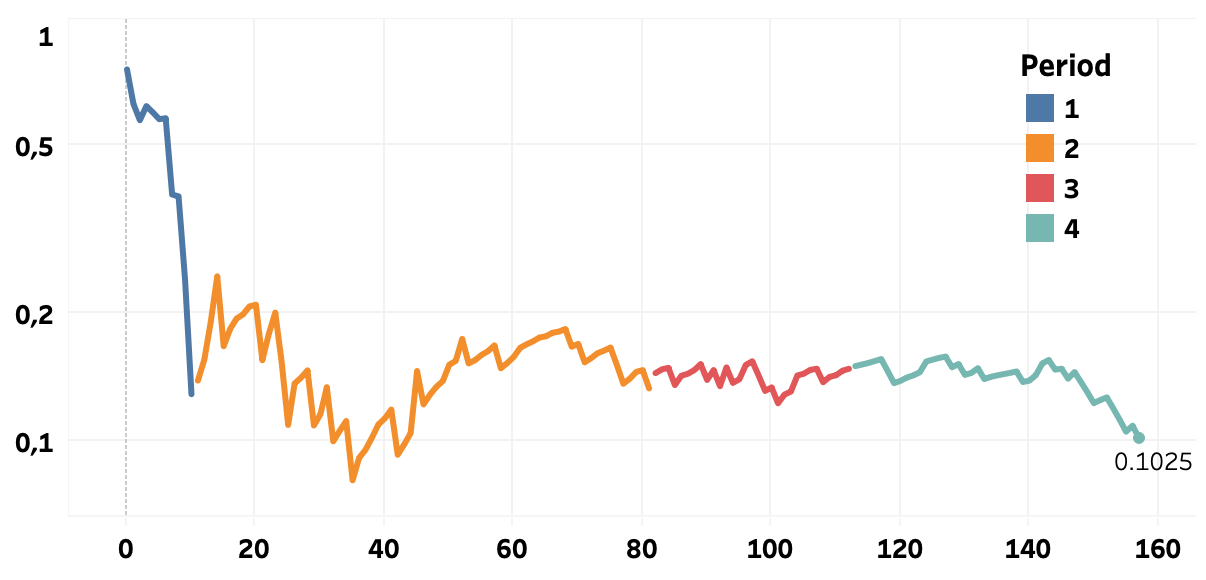
\includegraphics[width=\linewidth]{figures/pic2}
  \caption{Cumulative average profit over number of operations. An expected stabilization followed by a sudden decrease can be seen}
  \label{fig:chick}
\end{figure}

We can see in \autoref{fig:chick} that the data meets most of our expectations. However, we see the effects of the tendency change observed in Period 4. To put it in context, the change is so big in that region that even though there are more than 140 operations leading to a stable value, it still manages to draw it down a few points. Therefore the only remaining question now is: is that change actually significant? \\

The answer to that question can be found by performing a one-sided hypothesis test. For that we need to define our null and alternative hypothesis:

\begin{equation*}
    H_o \equiv \text{"The tendency in Period 4} \textbf{ isn't } \text{significantly lower"}
\end{equation*}
\begin{equation*}
    H_a \equiv \text{"The tendency in Period 4} \textbf{ is } \text{significantly lower"}
\end{equation*}

And we also need to set the confidence level (CL), which we will fix at $95\%$. That CL sets the $Z_c$ absolute value at $1.64$, so to reject our null hypothesis the calculated $Z$ absolute value must be higher. In our case we have:

\begin{equation*}
    |Z| = 2.49 > |Z_c|
\end{equation*}

So we can finally determine that the tendency change is significant. This implies that we should stop following our system's instructions until we clarify what's happening if we don't want to have further unexpected losses.

\subsection{Time dependence}

To examine the time dependence of our system we can put all our data together but separated in months to calculate the total profit for each month, as in \autoref{fig:clock}. Here we can see there are some good months, like November or February, and bad months like December or May, and in general we can see a pattern of two increments each followed by a decrease. However, \autoref{fig:clock} has been made mixing data from different periods so we have no assurance that it actually resembles how individual periods really perform. In order to determine if the identified pattern is reliable for predictions we need to compare it with every period separately.

\begin{figure}[hb]
  \centering
  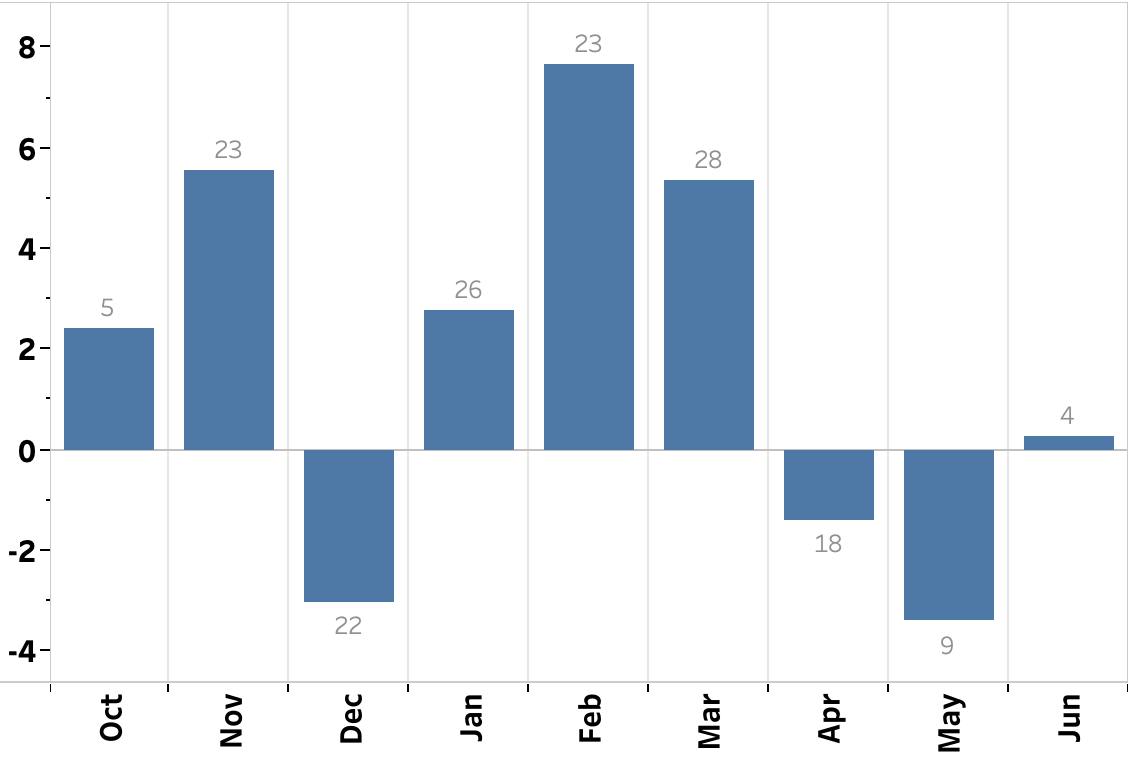
\includegraphics[width=\linewidth]{figures/pic3}
  \caption{Total profit by month. Numbers on the bars represent the number of operations recorded in the corresponding month}
  \label{fig:clock}
\end{figure}

In \autoref{fig:check} we have the total profit arranged by month and period. As we anticipated, there are some gaps that will make it harder to draw conclusions. Still, we can observe that the mentioned pattern is indeed present, although with some differences.

\begin{figure}[hb]
  \centering
  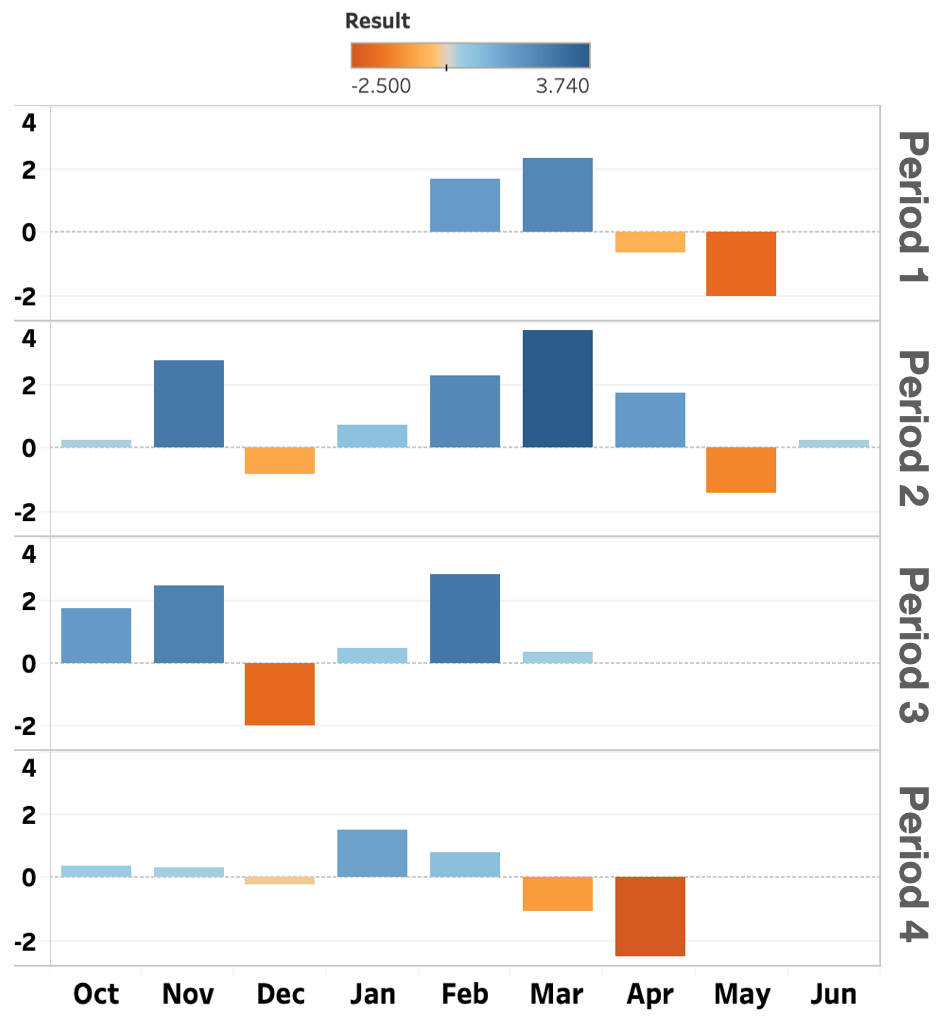
\includegraphics[width=\linewidth]{figures/pic4}
  \caption{Total profit by month and period.}
  \label{fig:check}
\end{figure}

We can see that December is consistently bad for investment and we also have the two increments before and after December. As for the second drop, we can see it is there, although it moves around so it would be harder to predict when exactly it will start in the future.\\

An interesting point here is that we might have found the reason why Period 4 is had such negative results. As we can see, in Period 4 the second drop happened way earlier than in previous periods, so we don't have enough good operations between the two drops to compensate for their negative values. In the future we could avoid this by not operating once we see we've entered the second drop.

\section{Conclusion}
After analyzing our data we can conclude that we have successfully found answers for our initial questions.\\

We have determined that there is a significant change in tendency during Period 4 and that has led us to a decision of stopping operations until the situation is clarified. However, we still don't know why this has happened or if the system will recover original tendency, although we have seen there is a connection with the system's temporal recursiveness that could help us avoid a similar situation in the future.\\

Furthermore, we have identified a pattern that seems to repeat, with slight differences, every period. That information can be used to avoid consistently bad months in order to optimize our system's performance.

\end{document}
\endinput
